\section{Diagramme de classe}

\begin{figure}[H]
  \center
  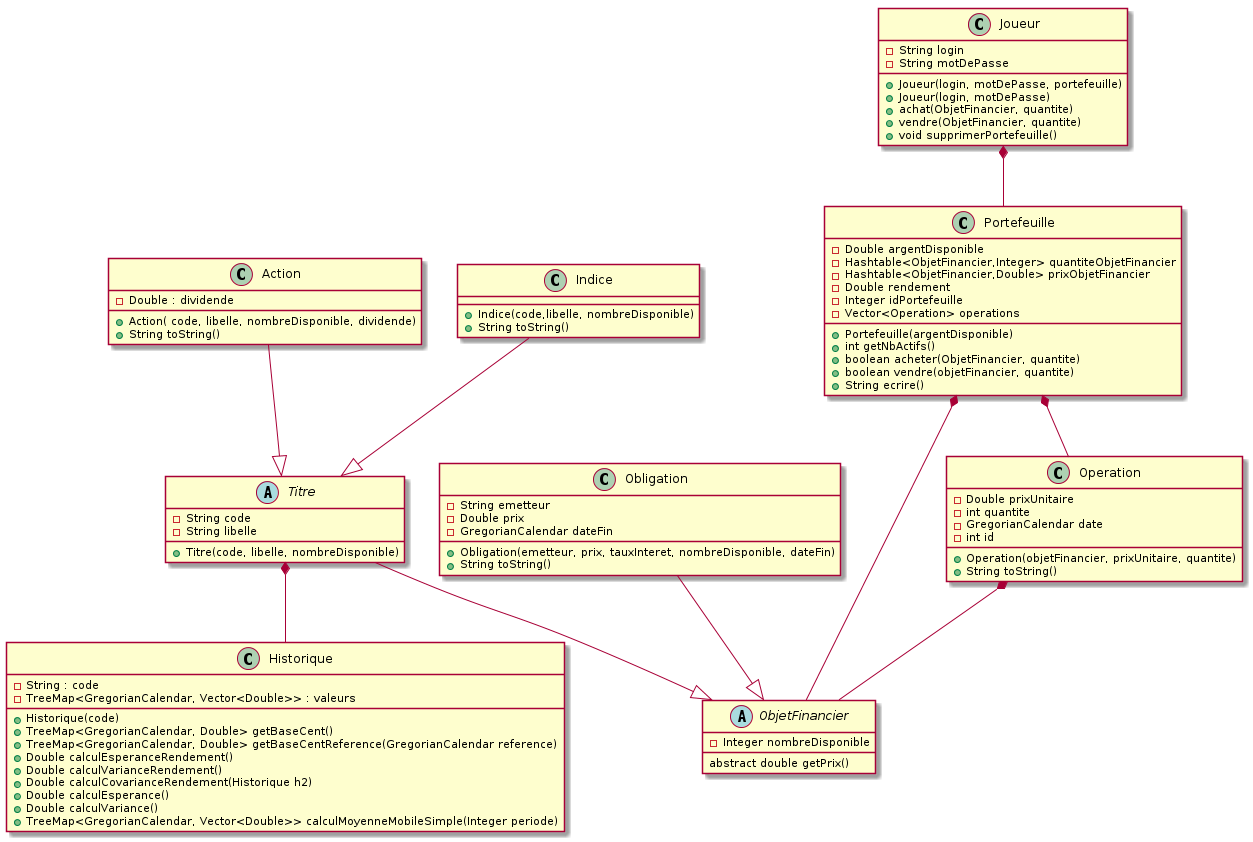
\includegraphics[scale=0.35]{../graph/DiagrammeClasseFinalModele.png} \\
  \caption{Diagramme de classe}
\end{figure}

Ce diagramme correspond au diagramme de classe général de notre partie modèle. Dans notre projet, un joueur possède un login et un mot de passe qu'il définit lors de son inscription ainsi qu'un portefeuille, il a la possibilité d'acheter un objet financier ou d'en vendre ainsi que de supprimer son portefeuille si la stratégie qu'il a employé jusqu'à présent ne le satisfait pas et qu'il veut recommencer. \\

\noindent Un portefeuille est constitué d'une somme d'argent disponible, de l’association entre un objet financier et une quantité d'une part ainsi qu'un prix d'autre part. Le portefeuille connaît également son id et la liste des opérations qu'il a effectué jusqu'à présent. Le portefeuille a la possibilité de réalisé un achat ou une vente. Il possède également la méthode écrire qui correspond à l'écrire au "format CSV" de notre portefeuille c'est-à-dire des différents composants du portefeuille (nom, prix, quantité) ainsi que la liste des opérations effectuées. \\

\noindent Une opération est composé d'un objet financier, un prix, une quantité et une date. \\

\noindent Un objetFinancier est une classe Abstraite qui généralise l'ensemble des objets financiers présents dans notre jeu. Un objet financier possède un nombre disponible sur le marché et un prix. On distingue deux types d'objet financiers. D'une part les obligations qui correspondent à un émetteur et une date de Fin et d'autre part les titres. Les titres sont eux mêmes abstraits, ils peuvent être spécialisés par les actions et les indices. Une action de distingue d'un indice par le dividende qu'il verse. Chaque titre possède un code et un libelle ainsi qu'un historique. \\

\noindent L'historique correspond à l'association pour chaque date de différentes valeurs pour notre titre, que ce soit la valeur d'ouverture, de fermeture, valeur la plus haute, la plus basse et les volumes. 